\documentclass[wide,a4paper,titlepage,12pt] {article}
\usepackage{polski}
\usepackage[utf8]{inputenc}
\usepackage{listings}
\usepackage{slashbox}
\usepackage[table]{xcolor}
\usepackage{graphicx,pdflscape}
\usepackage{placeins}
\usepackage{multirow}
\usepackage{slashbox}


\title{Projektowanie efektywnych algorytmów}
\author{Tymon Tobolski (181037)}

% Title page layout (fold)
\makeatletter
\renewcommand{\maketitle}{
\begin{titlepage}
  \begin{center}
    \vspace*{3cm}
    \LARGE \@title \par
    \vspace{2cm}
    \textit{\small Autor:}\par
    \normalsize \@author\par \normalsize
    \vspace{3cm}
    \textit{\small Prowadzący:}\par
    Mgr inż. Karolina Mokrzysz \par
    \vspace{2cm}
    Wydział Elektroniki\\ III rok\\ Pn TP 11.15 - 1.00\par
    \vspace{4cm}
    \small \@date
  \end{center}
\end{titlepage}
}
\makeatother
  \lstset{
    language=haskell,
    basicstyle=\ttfamily\scriptsize,
    numbers=left,
    numberstyle=\scriptsize,
    stepnumber=10,
    numbersep=9pt,
    showspaces=false,
    showstringspaces=false,
    showtabs=false,
    breaklines=true,
  }

\begin{document}
\maketitle
  \section{Cel projektu}
  \paragraph{}
  Celem projektu jest implementacja algorytmu rozwiązującego NP-trudny problem szeregowania n zadań na dwóch równoległych maszynach ($P_2||C_{max}$) przy pomocy wielomianowego schematu aproksymacyjnego PTAS.

  \section{Wielomianowy schemat aproksymacyjny}
  \paragraph{}
  Wielomianowy schemat aproksymacyjny (ang. PTAS - Polynomial-time approximation scheme) jest algorytmem aproksymacyjnym, pozwalającym na uzyskanie dowolnie dobrego rozwiązania przybliżonego danego problemu w czasie wielomianowym.

  \section{Algorytm}
  \paragraph{}
  Zaimplementowany algorytm składa się z kilku kroków:
  \begin{itemize}
    \item Posortowanie zadań malejąco po czasie wykonania
    \item Obliczenie wartości optymalnej
    \item Obliczenie górnego ograniczenia na podstawie wartości optymalnej i zadanego parametru $\varepsilon$
    \item Podzielenie zadań na dwie grupy względem wartości górnego ograniczenia
    \item Przyporządkowanie zadania z wartościami większymi za pomocą algorytmu dokładnego (przegląd zupełny)
    \item Przyporządkowanie pozostałych zadań za pomocą algorytmu przybliżonego (LPT)

    \newpage

    \section{Implementacja algorytmu}
    \paragraph{}

    \lstinputlisting{main.hs}

  \end{itemize}

  \section{Środowisko testowe}
  \paragraph{}
  Program testowy został napisany w języku Haskell przy pomocy kompilatora GHC w wersji 7.0.3.

  Testy zostały przeprowadzone na komputerze o poniższych parametrach:

  \begin{itemize}
    \item System operacyjny: Max OS X 10.7.1
    \item Procesor: 2.4 GHz Intel Core 2 Duo
    \item Pamięc RAM: 8 GB 1067 MHz
  \end{itemize}

  \section{Wyniki}
  \paragraph{}
  Uśredniony czas (w sekundach) wykonania 100.000 szeregowań w zależności od ilości zadań $n$ oraz parametru $\varepsilon$:

  \begin{center}
    \begin{tabular}{|c|c|c|c|c|}
      \hline
      \backslashbox{$\varepsilon$}{$n$} & 10 & 20 & 30 & 40 \\
      \hline
      0.04 & 1.03 & 1.39 & 2.67 & 4.07 \\
      \hline
      0.05 & 0.87 & 1.44 & 1.98 & 2.72 \\
      \hline
      0.06 & 0.92 & 1.47 & 1.94 & 2.44 \\
      \hline
      0.07 & 0.95 & 1.46 & 1.93 & 2.33 \\
      \hline
      0.08 & 0.84 & 1.41 & 1.78 & 2.31 \\
      \hline
      0.09 & 0.81 & 1.31 & 1.76 & 2.23 \\
      \hline
      0.10 & 0.79 & 1.32 & 1.71 & 2.19 \\
      \hline
      0.20 & 0.76 & 1.25 & 1.70 & 2.16 \\
      \hline
      0.30 & 0.76 & 1.38 & 1.80 & 2.16 \\
      \hline
    \end{tabular}
  \end{center}

  \begin{figure}[h!\texttt{}]
    \begin{center}
      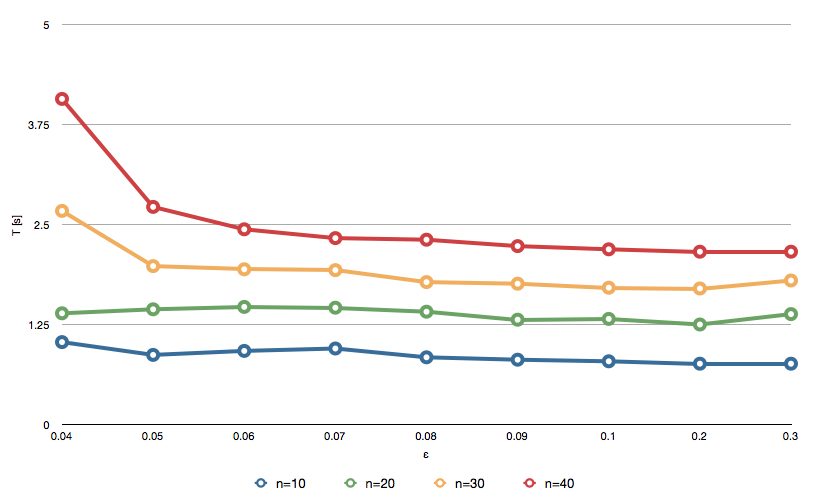
\includegraphics[width=\textwidth]{wyk.png}
      \caption{Czas potrzebny do wyznaczenia przybliżonego uszeregowania w zależności od $n$ i $\varepsilon$}
    \end{center}
  \end{figure}

  \paragraph{}
    Na Rysunku 1 przedstawiono zależność między parametrem $\varepsilon$, a czasem wykonania szeregowania dla czterech różnych długości listy zadań. Analizując wyniki testów można wnioskować, iż największy wpływ na czas szeregowania ma ilośc zadań. Na wykresie widać także, że czas szeregowania dla $\varepsilon$ należącego do przedziału $(0.06 - 0.3)$ nie różni się znacząco. Dopiero dla wartości $\varepsilon < 0.05$ widać znaczne spowolnienie algorytmu.


    \section{Wnioski}
    \paragraph{}
    W opracowanych przypadku PTAS jest swego rodzaju kompromisem pomiędzy przeglądem zupełnym, a algorytmem przybliżonym (LPT). Dzięki zastosowaniu schematu aproksymacyjnego uzyskane wyniki są lepsze niż przy zastosowaniu tylko algorytmu przybliżonego LPT lecz nadal gorsze niż w przypadku pełnego algorytmu dokładnego.
    \paragraph{}
    Wielomianowy schemat aproksymacyjny jest stosunkowo łatwą do zaimplementowania metodą uzyskiwania przybliżonych wyników skomplikowanych problemów optymalizacyjnych. Jak w wiekszości algorytmów przybliżonych rezultaty algorytmu zależą w dużej części od zadanych parametrów. W celu uzyskania dobrych wyników należy zadać małą wartość parametru $\varepsilon$, co oznacza dłuższy czas wykonania algorytmu i zbliża całość (w opracowanych przypadku) do przeglądu zupełnego.



\end{document}
